Using our newly constructed difference based extrapolation framework, we can now do the same analysis on our three nuclei \n{2}{H}, \n{3}{H} and \n{4}{He} using the same interaction as used earlier. Even though the difference based framework uses differences to compute a difference prediction internally, the final evaluation will still base off the same absolute energy differences and result in an absolute energy prediction. This means that we can apply our different evaluation modifications from \autoref{chap:extended} and discuss the influences of them on the difference based evaluation. Furthermore, using the same nuclei allows us to compare the difference based extrapolation and the absolute value extrapolation.

The results of our difference based extrapolation is shown in \autoref{fig:eval_diff}. The final extrapolated values and their uncertainty are shown in \autoref{tab:eval_diff} as well for each $N_\mathrm{max}$ and each SRG flow parameter.

% Generell: Predictions VIEL genauer, besonders bei hohem Nmax
Looking at all three nuclei, we can see that the uncertainty of all training modes is drastically reduced. Especially for higher $N_\mathrm{max}$, the predictions get very precise. Furthermore, the absolute value of the predictions are generally way closer to a reasonable limit. This can be seen for the nuclei \n{4}{He} and \n{3}{H}, where the networks trained with the unmodified or the $N_\mathrm{max}$-limitation training mode in the absolute based extrapolation framework predicted too low values for all $N_\mathrm{max}$. This could be caused by the fact that the absolute values are purged from the resulting differences, such that the absolute value of the sequences do not matter in the extrapolation process. This leads to a focus on the convergence of the sequences. When the sequence converges, the differences tend towards zero, such that evaluation yields a prediction for the ground-state energy close to the last values in the inputted sequences. We can see a disadvantage of the difference based extrapolation in the nucleus \n{4}{He} for a flow parameter of $\eta = \srg{0.04}$. Here, the sequences converge fast, but for the small values of $N_\mathrm{max}$ given, the sequences are cut off for the lower oscillator frequencies of $\hbar\Omega = \SI{12}{\mega\electronvolt}$ and \SI{14}{\mega\electronvolt}. This leads to the network recieving a broad range of differences, resulting in a greater uncertainty for the ground-state energy prediction. We can also see that this effect gets better for $\eta = \srg{0.08}$, where even the sequences for the lower oscillator frequencies are now visibly more converged to the limit.

% H2: 0.08 schlechter als 0.04

\begin{table}[H]
  \caption{Extrapolation results in \si[]{\mega\electronvolt} of the difference based framework for the nuclei \n{2}{H} \textbf{(a)}, \n{3}{H} \textbf{(b)} and \n{4}{He} \textbf{(c)}. For each interaction characterized by the flow parameter $\eta = \srg{0.04}, \srg{0.08}$, the final extrapolation results for the given $N_\mathrm{max}$ value is shown. Here, \textbf{(1)} is our basic extrapolation without further modifications of the training step, \textbf{(2)} is the $N_\mathrm{max}$-limitation training mode, \textbf{(3)} is the SRG-filter training mode. }
  \label{tab:eval_diff}
  \centering
  \begin{subtable}{\textwidth}
    \caption{}
    \centering
    \begin{tabular}{
        r|
        S[table-format=-2.3(3)]
        S[table-format=-2.3(3)]
        S[table-format=-2.3(3)]
        S[table-format=-2.3(3)]
        S[table-format=-2.3(3)]
        S[table-format=-2.3(3)]
      }
      \toprule
      $\eta$                           &
      \multicolumn{3}{c}{$\srg{0.04}$} &
      \multicolumn{3}{c}{$\srg{0.08}$}   \\
      \midrule
      $N_\mathrm{max}$                 &
      {8}                              &
      {10}                             &
      {12}                             &
      {8}                              &
      {10}                             &
      {12}                               \\
      \midrule
      (1)                              &
      -2.066 \pm 0.065                 &
      -2.144 \pm 0.025                 &
      -2.129 \pm 0.022                 &
      -2.054 \pm 0.069                 &
      -2.113 \pm 0.028                 &
      -2.126 \pm 0.023                   \\
      (2)                              &
      -2.080 \pm 0.055                 &
      -2.146 \pm 0.023                 &
      -2.127 \pm 0.020                 &
      -2.064 \pm 0.056                 &
      -2.110 \pm 0.026                 &
      -2.124 \pm 0.022                   \\
      (3)                              &
      -2.068 \pm 0.055                 &
      -2.153 \pm 0.038                 &
      -2.149 \pm 0.034                 &
      -2.062 \pm 0.041                 &
      -2.124 \pm 0.032                 &
      -2.158 \pm 0.036                   \\
      \bottomrule
    \end{tabular}
  \end{subtable}
  \par\bigskip
  \begin{subtable}{\textwidth}
    \caption{}
    \centering
    \begin{tabular}{
        r|
        S[table-format=-2.3(3)]
        S[table-format=-2.3(3)]
        S[table-format=-2.3(3)]
        S[table-format=-2.3(3)]
        S[table-format=-2.3(3)]
        S[table-format=-2.3(3)]
      }
      \toprule
      $\eta$                           &
      \multicolumn{3}{c}{$\srg{0.04}$} &
      \multicolumn{3}{c}{$\srg{0.08}$}   \\
      \midrule
      $N_\mathrm{max}$                 &
      {8}                              &
      {10}                             &
      {12}                             &
      {8}                              &
      {10}                             &
      {12}                               \\
      \midrule
      (1)                              &
      -8.453 \pm 0.099                 &
      -8.528 \pm 0.044                 &
      -8.470 \pm 0.026                 &
      -8.410 \pm 0.090                 &
      -8.465 \pm 0.035                 &
      -8.460 \pm 0.025                   \\
      (2)                              &
      -8.461 \pm 0.082                 &
      -8.526 \pm 0.036                 &
      -8.468 \pm 0.025                 &
      -8.422 \pm 0.074                 &
      -8.464 \pm 0.031                 &
      -8.457 \pm 0.023                   \\
      (3)                              &
      -8.390 \pm 0.064                 &
      -8.493 \pm 0.028                 &
      -8.466 \pm 0.026                 &
      -8.408 \pm 0.045                 &
      -8.460 \pm 0.026                 &
      -8.466 \pm 0.025                   \\
      \bottomrule
    \end{tabular}
  \end{subtable}
  \par\bigskip
  \begin{subtable}{\textwidth}
    \caption{}
    \centering
    \begin{tabular}{
        r|
        S[table-format=-2.3(3)]
        S[table-format=-2.3(3)]
        S[table-format=-2.3(3)]
        S[table-format=-2.3(3)]
        S[table-format=-2.3(3)]
        S[table-format=-2.3(3)]
      }
      \toprule
      $\eta$                           &
      \multicolumn{3}{c}{$\srg{0.04}$} &
      \multicolumn{3}{c}{$\srg{0.08}$}   \\
      \midrule
      $N_\mathrm{max}$                 &
      {8}                              &
      {10}                             &
      {12}                             &
      {8}                              &
      {10}                             &
      {12}                               \\
      \midrule
      (1)                              &
      -28.502 \pm 0.397                &
      -28.497 \pm 0.212                &
      -28.405 \pm 0.095                &
      -28.520 \pm 0.175                &
      -28.535 \pm 0.064                &
      -28.529 \pm 0.025                  \\
      (2)                              &
      -28.399 \pm 0.319                &
      -28.454 \pm 0.177                &
      -28.391 \pm 0.080                &
      -28.522 \pm 0.143                &
      -28.537 \pm 0.052                &
      -28.530 \pm 0.021                  \\
      (3)                              &
      -28.377 \pm 0.294                &
      -28.408 \pm 0.139                &
      -28.353 \pm 0.054                &
      -28.507 \pm 0.065                &
      -28.521 \pm 0.026                &
      -28.527 \pm 0.012                  \\
      \bottomrule
    \end{tabular}
  \end{subtable}
\end{table}


Another effect of the difference based extrapolation is that the different training modes now generally predict a ground-state energy in the same range. However, now the impact of the training modes has shifted from the absolute value of the prediction into the uncertainty of the prediction. This can be seen especially for the SRG-filter training mode, where the uncertainty generally gets smaller for the nuclei \n{3}{H} and \n{4}{He}, but larger for \n{2}{H}, which can be attributed to the slow convergence of \n{2}{H} sequences.
For the first and second training mode of the \n{2}{H} nucleus, we can also observe that the difference based framework produces a smaller uncertainty than the range of the classical extrapolations.

For \n{2}{H} and \n{3}{H}, we can also see that the predictions for the ground-state energy are a bit higher for the SRG flow parameter of \srg{0.08} than \srg{0.04}.

Note that the difference based extrapolation framework is not completely independent on the absolute values of the sequences, since the prediction target for the network training is calculated using the average of the absolute values for the highest $N_\mathrm{max}$. This can also result in a dependency on the spread of the different sequences for the evaluated maximum $N_\mathrm{max}$.

\begin{figure}[H]
  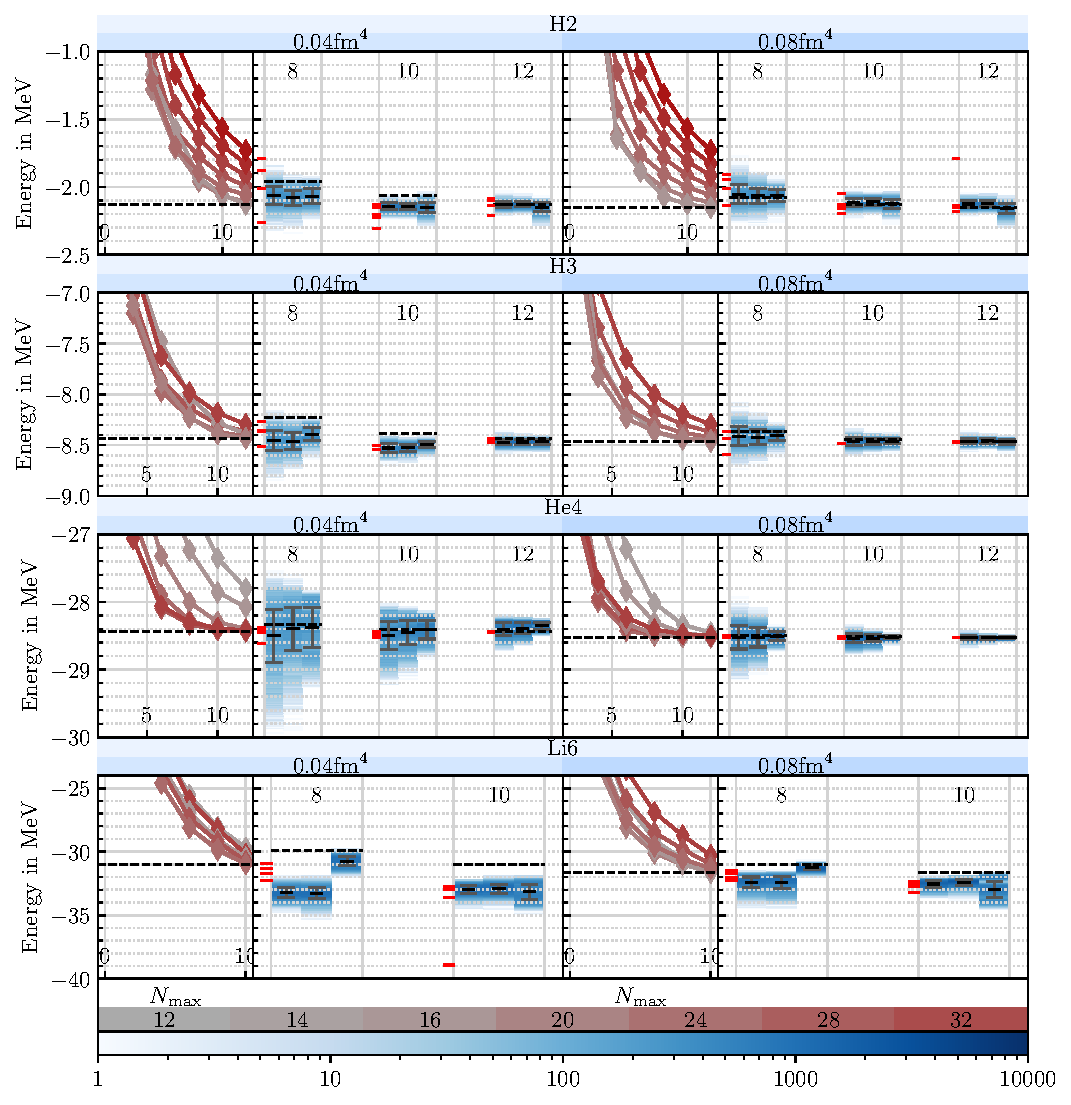
\includegraphics[width=\textwidth]{media/diff_evaluation.pdf}
  \caption{Evaluation of our training modes on the nuclei of \n{2}{H}, \n{3}{H} and \n{4}{He} in the difference based extrapolation framework. The shown training modes are, in order from left to right, the basic training mode for comparison, the $N_\mathrm{max}$-limitation training mode and the SRG-filter training mode. For each nucleus and each flow parameter, the NCSM sequences are shown on the left and the extrapolations for a given maximum $N_\mathrm{max}$ on the right. For each maximum $N_\mathrm{max}$, the variational boundary is shown as a dotted line, and the classical extrapolations are shown as red ticks.}
  \label{fig:eval_diff}
\end{figure}

